\documentclass{math}

\usepackage{tikz}

\title{CSCI 251: Concepts of Parallel and Distributed Systems}
\author{Alvin Lin}
\date{October 30th, 2017}

\begin{document}

\maketitle

\section*{Coordination and Agreement}
Topics:
\begin{itemize}
  \item Mutual Exclusion
  \item Election
  \item Multicast
\end{itemize}

\subsection*{Mutual Exclusion}
Requirements:
\begin{itemize}
  \item Safety: at any time, only one process has access to a critical section
  \item Livencess: a process making a request for access to a critical section,
  will eventually get access
  \item HB order (happened before order): entry to a critical section is in
  ``happened before'' order. A process \( P_i \) that makes a request before
  process \( P_j \) should get access before process \( P_j \)
\end{itemize}
Performance:
\begin{itemize}
  \item Bandwidth Consumption: number of messages sent on communication channels
  \item Client Delay: Amount of time a process waits after making a request
  \item Throughput: Number of requests granted per unit time
\end{itemize}

\subsection*{Client Server Mechanisms}
A server that receives requests from processes grants access to them one at a
time. The server maintains a queue to give access (first in first out).

\subsection*{Multicast}
A process can be in one of three states:
\begin{center}
  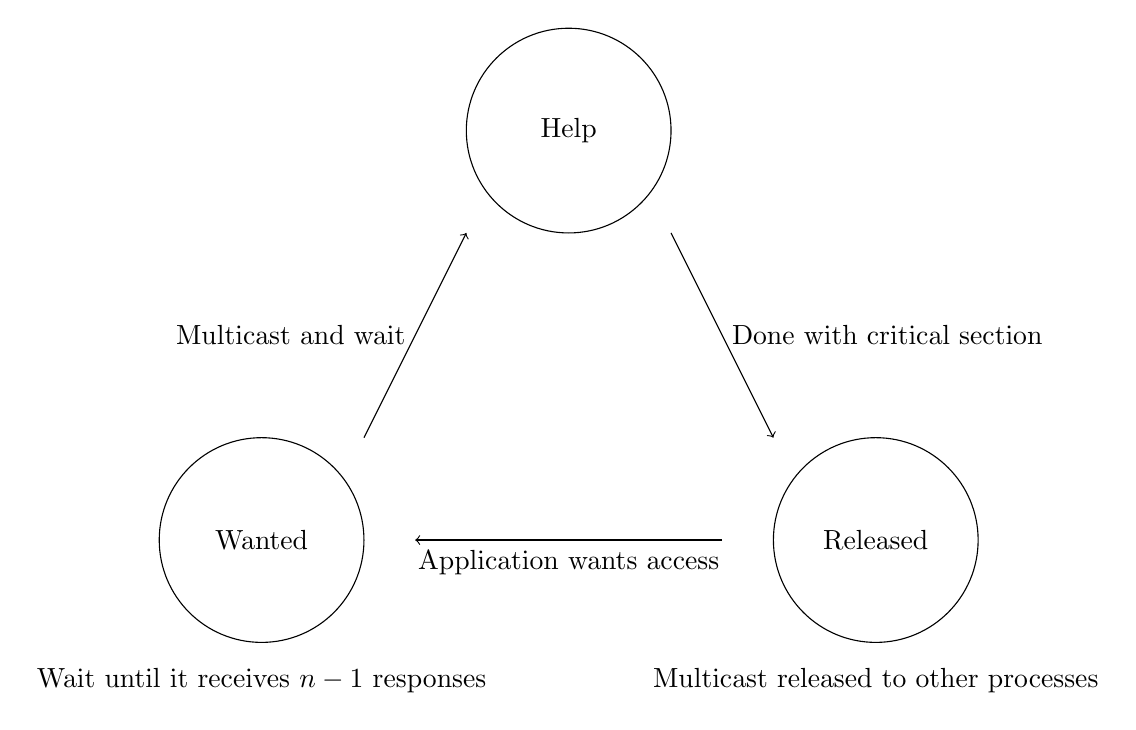
\begin{tikzpicture}[scale=1.3]
    \draw (0,4) circle (1cm) node {Help};
    \draw[->] (1,3) -- (2,1) node[pos=0.5,right] {Done with critical section};
    \draw (3,0) circle (1cm) node {Released}
      node[below,yshift=-1.5cm] {Multicast released to other processes};
    \draw[->] (1.5,0) -- (-1.5,0)
      node[pos=0.5,below] {Application wants access};
    \draw (-3,0) circle (1cm) node {Wanted}
      node[below,yshift=-1.5cm] {Wait until it receives \( n-1 \) responses};
    \draw[->] (-2,1) -- (-1,3) node[pos=0.5,left] {Multicast and wait};
  \end{tikzpicture}
\end{center}

\subsection*{Election Algorithm}
In distributed systems, it is necessary to select a leader among a set of
processes to assign tasks to processes, to make decisions, and decide on
variables. Any process in the system can decide whether a leader needs to be
elected. This can happen by agreement when process \( p_i \) initiates the
election process designating \( p_j \) as the leader and sends a multicast
to all other processes. Other processes can agree or disagree, in which case
the processes suggests another leader process and multicasts.

\section*{Reminders}
Check MyCourses for details on Project 2. \\
\noindent Professor Mohan Kumar: \\
\url{mjkvcs@rit.edu} \\
\url{https://cs.rit.edu/~mjk} \\

\noindent Rahul Dashora (TA): \\
\url{rd5476@mail.rit.edu} \\

\begin{center}
  You can find all my notes at \url{http://omgimanerd.tech/notes}. If you have
  any questions, comments, or concerns, please contact me at
  alvin@omgimanerd.tech
\end{center}

\end{document}
